\newpage

\section{Soft constraints}

I vincoli soft permettono di associare un \textbf{livello di preferenza} a
ciascun assegnamento di valori per una tupla.

Questo implica che non ci sono più solo due livelli di soddisfacibilità
(0 e 1), ma molti altri\dots\\

\textbf{Esempio}: si vuole decidere cosa mangiare in un ristorante, dato
un certo menù. Si possono avere delle preferenze sui singoli piatti o
bevande e sulla loro combinazione. Si cerca il pasto che massimizzi
la preferenza di un cliente.

Un \textbf{vincolo soft} è simile a un vincolo classico, dove ciascun
assegnamento di valori alle variabili è associato a un valore di
preferenza (appartenente a un insieme parzialmente ordinato).

La figura \ref{fig:soft} mostra un vincolo soft per il problema del
ristorante.

\begin{figure}[H]
\centering
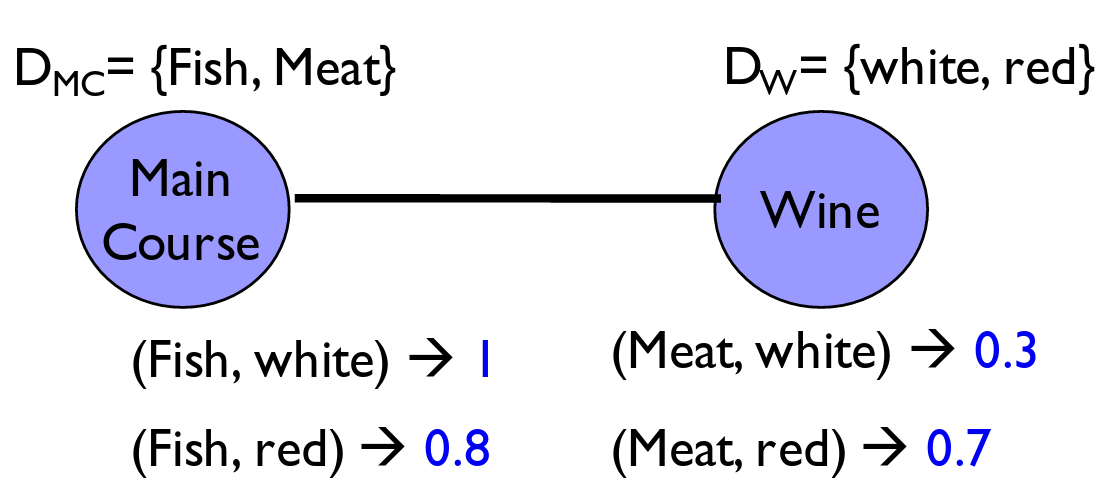
\includegraphics[width=0.5\textwidth]{soft}
\caption{Esempio di vincolo soft per l'esempio del ristorante}
\label{fig:soft}
\end{figure}

L'insieme parzialmente ordinato dei valori di preferenza ha 2 operazioni e
questo lo rende simile a un semianello. Si basa sulla struttura
\textbf{c-semianello}.

\subsection{Formalismo del c-semianello}

Sia $<A, +, *, 0, 1>$ un semianello:

\begin{itemize}
 \item A è l'insieme dei valori di preferenza
 \item + è l'operazione di proiezione
 \item * è l'operazione di combinazione
 \item 0 è l'elemento che corrisponde al peggior valore di preferenza $0 \in A$
 \item 1 è l'elemento che corrisponde al miglior valore di preferenza $1 \in A$
\end{itemize}
